\documentclass[a4paper,12pt]{report}
\usepackage{acro}
\usepackage{array}
\usepackage{biblatex}
\usepackage{float}
\usepackage{graphicx}
\usepackage{hyperref}
\usepackage{indentfirst}
\usepackage[utf8]{inputenc}
\usepackage{listings}
\usepackage{xcolor}

\definecolor{codegreen}{rgb}{0,0.6,0}
\definecolor{codegray}{rgb}{0.5,0.5,0.5}
\definecolor{codepurple}{rgb}{0.58,0,0.82}
\definecolor{backcolour}{rgb}{0.95,0.95,0.92}

\lstdefinestyle{codestyle}{
    backgroundcolor=\color{backcolour},   
    commentstyle=\color{codegreen},
    keywordstyle=\color{magenta},
    numberstyle=\tiny\color{codegray},
    stringstyle=\color{codepurple},
    basicstyle=\ttfamily\footnotesize,
    breakatwhitespace=false,         
    breaklines=true,                 
    captionpos=b,                    
    keepspaces=true,                 
    numbers=left,                    
    numbersep=5pt,                  
    showspaces=false,                
    showstringspaces=false,
    showtabs=false,                  
    tabsize=2
}

\lstset{style=codestyle}

\DeclareAcronym{cfi}{
  short = CFI,
  long  = Control-Flow Integrity,
  tag = abbrev
}
\DeclareAcronym{cfg}{
  short = CFG,
  long  = Control-Flow Graph,
  tag = abbrev
}
\DeclareAcronym{dfc}{
  short = DFC,
  long  = direct function calls,
  tag = abbrev
}
\DeclareAcronym{ifc}{
  short = IFC,
  long  = indirect function calls,
  tag = abbrev
}
\DeclareAcronym{lto}{
  short = LTO,
  long  = Link-time Optimization,
  tag = abbrev
}
\DeclareAcronym{llvm-ir}{
  short = LLVM IR,
  long  = LLVM Intermediate Representation,
  tag = abbrev
}
\DeclareAcronym{rtti}{
  short = RTTI,
  long  = Run-time Type Information,
  tag = abbrev
}


\addbibresource{main.bib}
\setlength{\parskip}{0.5em}
\renewcommand{\baselinestretch}{1.15}

\title{
\includegraphics[keepaspectratio,width=0.5\paperwidth]{img/hku.png} \\ Refining Function Pointers’ Targets With\\ Class Hierarchy Tree Reconstruction and Object-Flow Analysis\\ \  \\Progress Report 1}
\author{Binrui Dong\\ (3035534816)\\ \ \\ Supervisor\\ Chenxiong Qian}
\date{\today}

\begin{document}

\maketitle

\newpage
\chapter*{Abstract}
\label{chapter:abstract}
\addcontentsline{toc}{chapter}{\nameref{chapter:abstract}}

Control-Flow Integrity (CFI) is a technique to protect software programs from being taken-over the execution path by a malicious attacker. It relies on building Control-Flow Graph (CFG) ahead of time which analyzes legitimate targets of each function call, but in practice the problem is complicated by indirect calls through function pointers, whose targets are not known in static analysis. This project proposes a new approach to analyze targets of indirect call through function pointers in C++ programs by class hierarchy tree reconstruction and object-flow analysis, in the hope that it could produce more accurate results compared to previous approaches. The project is currently in work-in-progress stage. Scaffolding code on loading LLVM bitcode files and reading their LLVM IR has been successfully completed. The next steps includes system and algorithm design, as well as more literature review on related topics.

\chapter*{Acknowledgments}
\label{chapter:acknowledgments}
\addcontentsline{toc}{chapter}{\nameref{chapter:acknowledgments}}

I would like to thank the supervisor, Dr. Chenxiong Qian, for mentoring me and supporting the project from its very beginning.

I also greatly appreciate the help of Miss Mable Choi for her attentive guidance in the language and organization of this final year project progress report.

\newpage

\tableofcontents

\newpage

\listoffigures
\addcontentsline{toc}{chapter}{List of Figures}

\listoftables
\addcontentsline{toc}{chapter}{List of Tables}

\printacronyms[include=abbrev,name=Abbreviations]
\addcontentsline{toc}{chapter}{Abbreviations}

\newpage
\chapter{Introduction}

\section{Background}
\label{section:background}

To date, many large modern software are written in C/C++ programming languages, from operating system kernels such as Linux and FreeBSD, to user space applications, including databases (e.g. MySQL, MongoDB), web browsers (e.g. Firefox, Chromium) and video game engines (e.g. Unreal Engine).

C/C++ allows programmers to directly manipulate memory, which helps in building high performance software programs, however, it also leaves door open for potential security vulnerabilities \cite{BurowNathan2017CIPS}. Attackers may make use of oversights in the program (such as omission of input validation, array bounds checking, etc.) to corrupt memory, and divert the control-flow of the program away from its original legitimate region to execute malicious code.

\begin{figure}[ht]
    \centering
    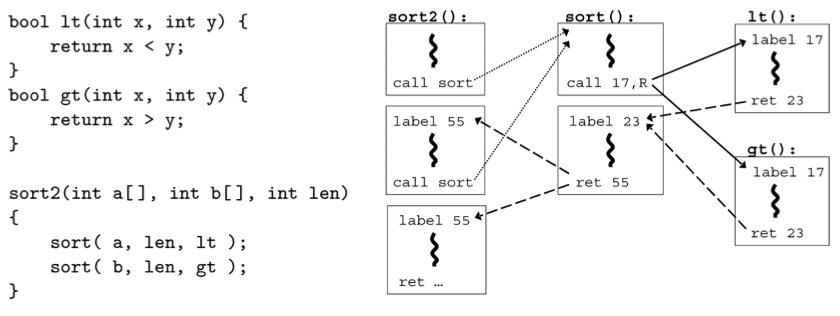
\includegraphics[keepaspectratio,width=0.65\paperwidth]{img/cfg.png}
    \caption{A piece of C code on the left, and its Control-Flow Graph \cite{cfi2005}.}
    \label{fig:cfg}
\end{figure}

In response, \ac{cfi} technique \cite{cfi2005} attempts to safeguard a program by restricting the control-flow of the program to its valid space \cite{nebelwelt}. The technique is composed of two phases, an ahead-of-time \textbf{analysis phase}, and a run-time \textbf{enforcement phase} \cite{BurowNathan2017CIPS}.

During analysis phase, static analysis is performed on source code or binary of the program to compute its \ac{cfg}, which basically represents the set of legitimate control-flow state transfers, such as function calls and returns.

Figure \ref{fig:cfg} illustrates an example of a control-flow graph. On the left, there is a piece of C code that contains three functions, \texttt{sort2()}, \texttt{lt()} and \texttt{gt()}. On the right is the control-flow graph of the source code. Nodes on the graph refer to functions in the program, and edges represent legitimate jumping from a location in a function to another location in another function.

More specifically, solid line arrows in the figure are called ``forward edge'', which represents a function call operation, where during the execution of a parent function, a child function is invoked and the program transfers to the child function. Dashed line arrows are called ``backward edge'', representing a return operation, where the child function returns to the parent caller function.

The control-flow graph in the figure illustrates that function \texttt{sort2()} may call function \texttt{sort()} at two locations in the middle of \texttt{sort2()}, and function \texttt{sort()} may call function \texttt{lt()} and function \texttt{gt()} in the middle of \texttt{sort()}. At the end of each children functions \texttt{sort()}, \texttt{lt()} and \texttt{gt()}, there is a backward edge returning to their parent call site.

After control-flow graph is constructed, during run-time enforcement phase, each control-flow state transfer is verified by checking whether there exists such an edge in CFG. If the transfer does not exist in the pre-computed CFG, then the control-flow integrity of the program must have been compromised, and actions can be taken, for example, terminate the program execution, send an alert to users and administrators, etc.

\section{Motivation}
\label{section:motivation}

Constructing control-flow graphs for programs like the one illustrated in Figure \ref{fig:cfg} is simple, because it only contains \ac{dfc}. Here ``direct function call'' refers to calling a function by its name, such as \texttt{memcpy(a, b, n);} and \texttt{fopen("file.txt", "r");}. In this case, it is sufficient to simply generate forward edges to \texttt{memcpy()} and \texttt{fopen()}, and backward edges returning to the paren caller function.

However, constructing control-flow graphs is much more complicated in the presence of \ac{ifc}. Indirect function calls are call operations to memory addresses instead of static function names. For instance, calling through a function pointer is an indirect function call.

Figure \ref{fig:fptr} illustrates an example of such a scenario. In the body of function \texttt{funcX()}, there is an indirect function call \texttt{p(2, 3);}, where \texttt{p} is not a function, but a function pointer. In this situation, static analysis is unable to immediately determine what is the target of the function call \texttt{p(2, 3);}, and hence unable to generate the control-flow graph for the program in Figure \ref{fig:fptr}.

\begin{figure}[h]
    \centering
    \begin{lstlisting}[language=c]
// Defines function pointer type
typedef int (*fptr_t)(int, int);

// Defines two functions of the type
int funcA(int a, int b) { return a + b; }
int funcB(int a, int b) { return a * b; }

// An indirect call happens here
int funcX(fptr_t p) { return p(2, 3); }

int main() { return funcX(&funcA); }
    \end{lstlisting}
    \caption{An example of function pointers and indirect function call}
    \label{fig:fptr}
\end{figure}

\newpage

Function pointers are extensively used in practical software development. For example, in Linux kernel, in order to support \texttt{open()} system call on different file-systems, the kernel may store function pointers to the underlying implementations of such functionality for \texttt{ext4}, \texttt{xfs}, \texttt{btrfs}, etc., and dynamically invoke the corresponding underlying function during run-time depending on the file-system used \cite{mlta}.

Function pointers are even essential in C++ language to realize run-time polymorphism. Objects of different subclass types can be passed as pointers or references in their common superclass type, but when calling a virtual method of the superclass type, the overriden method implementations of each respective subclass are actually called. This is achieved by each class object maintaining a virtual function table that stores function pointers to the actual method implementations of the concrete type of the object. During run-time, when calling a virtual method of the class object, the program queries its virtual function table for the memory address of the method implementation to be called, and calls the method through this function pointer.

In order for control-flow integrity to be practically useful in real-world applications, indirect function calls have to be handled properly. Control-flow integrity without support for indirect function calls is like a safety net with holes here and there, where direct function calls are verified and protected, but indirect function calls are totally exposed unprotected. Study shows that the constructed control-flow graph is often erroneously too small and barely useful, if function pointers are ignored \cite{cfg-extract}.

If call targets of indirect function calls are captured in control-flow graphs, then control-flow integrity enforcement can also cover indirect function calls, so that the effectiveness of control-flow protection is greatly improved. However, this is a hard problem, and in practice it is almost impossible to find call targets of indirect function calls in one hundred percent accuracy. Nonetheless, it is desirable to resolve targets of indirect function calls as precisely as possible, so the effectiveness of control-flow integrity enforcement is better than not covering indirect function calls at all, while not causing much performance overhead. Chapter \ref{chapter:previous-work} presents some of the existing approaches in doing so.

\section{Objective}
\label{section:objective}

This project aims to more accurately refine targets of indirect calls on function pointers, in the context of control-flow graph construction in C++ programs.

The scope of this project includes system and algorithm design, code implementation, results evaluation and comparison to other approaches.

In the end, this project will deliver a static analysis tool that performs function pointer targets analysis on C++ programs.

\section{Report Outline}
\label{section:outline}

The structure of this report in the following sections is organized as follows. Chapter \ref{chapter:previous-work} discusses some of the previous work in the field of analyzing the targets of indirect calls through function pointers in software programs, including simple type matching, and the state-of-the-art approach called multi-layer type analysis. Chapter \ref{chapter:methodology} introduces the methodology used in the project. Chapter \ref{chapter:status} presents current project status. Finally, chapter \ref{chapter:conclusion} concludes this project progress report in the end.

\newpage
\chapter{Previous Work}
\label{chapter:previous-work}

Two categories of current existing approaches in identifying targets of indirect function calls, namely Pointer Analysis and Type Analysis, are introduced in section \ref{section:pointer-analysis} and section \ref{section:type-analysis}. A novel method called Multi-Layer Type Analysis is then introduced in section \ref{section:mlta}.

\section{Pointer Analysis}
\label{section:pointer-analysis}

Pointer analysis, also called points-to analysis, attempts to compute the set of memory addresses that a pointer may possibly point to, by the means of static analysis  \cite{hind2001pointer}. With this information available, control-flow graphs at function pointer indirect calls can be constructed by extending forward edges to all functions that the pointer may point to, and also generating backward edges that represents return operations.

However, studies show that perfectly precise pointer analysis is in general undecidable \cite{undecidability-of-aliasing} \cite{undecidability-of-static-analysis} , meaning that it is not feasible to accurately determine the exact set of memory addresses a pointer may point to without any omission nor over-approximation.

Therefore, in order for pointer analysis to be practical, precision has to be sacrificed in favor of reasonable analysis time efficiency \cite{jujutsu}. There are a number of approximation algorithms offering various trade-offs between accuracy and time efficiency, with worst case time complexities ranging from linear to exponential \cite{hind2001pointer}. But it has been demonstrated that the imprecision due to conservative over-approximation can lead to successful security exploit even when \ac{cfi} is enforced \cite{jujutsu}, which severely undermines the effectiveness of \ac{cfi}.

\section{Type Analysis}
\label{section:type-analysis}

The basic idea of type analysis is filtering the set of possible call targets of a function pointer indirect call by function type information. Functions with the same type as the function pointer are considered possible call targets.

Niu and Tan \cite{modular-cfi} propose control-flow graph construction with type analysis, and they implement their approach in a modified LLVM compiler. Auxiliary type information of functions and function pointers is annotated to intermediate representation of compilation units along with code and data. When generating control-flow graphs at a function pointer indirect call, forward edges are extended to functions with the same type.

A simplified variant of type analysis is implemented in LLVM compiler \cite{ifcc}, called ``Indirect Function Call Check (IFCC)''. It analyzes LLVM IR during \ac{lto} stage of compilation. Instead of checking function types, it only checks whether the number of parameters of a function matches with the function pointer. This is relatively easier to implement and has less performance impact.

A down side of this approach is potentially large amount of false positives. Functions which are never called in the normal execution path are also reported, only because they have the same type. This problem is called type collision.  Farkhani et al. \cite{effectiveness-type-cfi} shows that type collision is fairly common in real-world large applications, and could be exploited by a malicious adversary to attack the program.

\section{Multi-Layer Type Analysis}
\label{section:mlta}

Lu and Hu \cite{mlta} propose a novel approach in function pointers target analysis called Multi-Layer Type Analysis on the 26-th ACM Conference on Computer and Communications Security in 2019.

This approach attempts to improve the accuracy of resolving indirect call target functions by looking into the multi-layer type hierarchy information of the chain of \texttt{struct}s or \texttt{class}s in which the function pointer is stored.

\begin{figure}[hb]
    \centering
    \begin{lstlisting}[language=c]
// Defines function pointer type
typedef int (*fptr_t)(int, int);

// Defines two functions of the type
int funcB(int a, int b) { return a + b; }
int funcC(int a, int b) { return a * b; }

// Defines three structs
struct A { fptr_t p; };
struct B { struct A a; };
struct C { struct A a; };

// Defines two instances of structs
struct B b = { .a = { .p = &funcB } };
struct C c = { .a = { .p = &funcC } };

int main() { return c.a.p(2, 3); }
    \end{lstlisting}
    \caption{Code example of Multi-Layer Type Analysis}
    \label{fig:mlta}
\end{figure}

In a simplified example illustrated in Figure \ref{fig:mlta}, for the indirect call \texttt{c.a.p()} in \texttt{main()} function, the function pointer \texttt{p} is stored in a \texttt{struct} of type \texttt{A}, which is in turn stored in a parent \texttt{struct} of type \texttt{C}. Then the scope of possible target functions for this indirect call is limited to those functions whose address are stored to pointers with the same multi-layer type hierarchy information, that is, function pointers that are also stored in a \texttt{struct} of type \texttt{A} in a parent \texttt{struct} of type \texttt{C}. In the example in Figure \ref{fig:mlta}, the only function satisfying such condition is \texttt{funcC}, since its address is stored to a \texttt{struct} of type \texttt{A} in a parent \texttt{struct} of type \texttt{C} at line 15. Although funciton \texttt{funcB} also has the same function type (taking two \texttt{int} parameters and returns an \texttt{int} value), the address of \texttt{funcB} is never assigned to a \texttt{struct} of type \texttt{A} in a parent \texttt{struct} of type \texttt{C}.

This approach is based on the intuition that in practical software development, function pointers are often stored in multi-layer objects of objects \cite{mlta}, and this is indeed effective in field test. The authors evaluate their technique on three real-world system programs, Linux, FreeBSD and Firefox, and observed 86\% to 98\% reduction in the target functions reported for indirect calls \cite{mlta}.

\section{Summary}
\label{section:previous-work-summary}

This chapter presents an overview of two categories of current existing approaches in resolving targets of indirect function calls, and a newly proposed approach as well. In the next chapter, methodology applied in the project is discussed.

\newpage
\chapter{Methodology}
\label{chapter:methodology}

This chapter first introduces the technology stack chosen that this project will be built upon in section \ref{section:llvm}, then discuss the two core methodologies used by the project, class hierarchy tree reconstruction, and object-flow analysis, in section \ref{section:class-tree} and section \ref{section:object-flow} respectively. Finally, evaluation of the work is discussed in section \ref{section:evaluation}.

\section{LLVM}
\label{section:llvm}

LLVM is a compiler and toolchain technologies framework \cite{llvm-website} composed of a collection of projects, most notably are

\begin{itemize}
    \item Clang, an optimizing C/C++/Objective-C compiler
    \item LLVM Core, a set of libraries offering architecture independent optimization and code generation support for different CPU architectures
\end{itemize}

These components are designed to work closely with \ac{llvm-ir}, an architecture and programming language independent form of software programs. It is similar to assembly language, in the sense that a piece of program in LLVM IR form is also composed of instructions that have operations and operands, but LLVM IR is portable across different CPU architectures, and preserves certain high-level language information, such as strong types and functions \cite{llvm-ir}.

\begin{figure}[H]
    \centering
    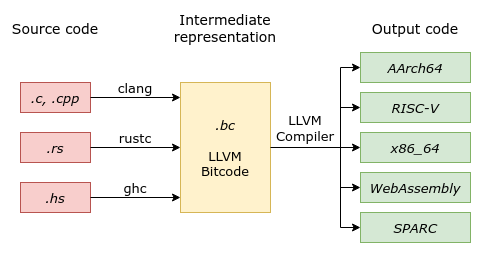
\includegraphics[keepaspectratio,width=0.6\paperwidth]{img/llvm-compiler.png}
    \caption{LLVM Compiling Pipeline \cite{llvm-pipeline}}
    \label{fig:llvm-compiler}
\end{figure}

\begin{figure}[H]
    \centering
    \begin{lstlisting}[language=c]
double square(double num) {
    return num * num;
}
    \end{lstlisting}
    \begin{lstlisting}[language=llvm]
define dso_local double @_Z6squared(double %0) local_unnamed_addr #0 {
  %2 = fmul double %0, %0
  ret double %2
}
    \end{lstlisting}
    \begin{lstlisting}[language={[x86masm]Assembler}]
square:
    sub     esp, 12
    movsd   xmm0, qword ptr [esp + 16]
    mulsd   xmm0, xmm0
    movsd   qword ptr [esp], xmm0
    fld     qword ptr [esp]
    add     esp, 12
    ret
    \end{lstlisting}
    \caption{a C++ function, its LLVM IR, and its x86 assembly code}
    \label{fig:llvm-ir}
\end{figure}

Figure \ref{fig:llvm-compiler} shows the process of compiling a program from source code to a binary executable that is runnable on a target architecture in LLVM. The compiler, Clang for C/C++ programs or \texttt{rustc} for Rust programs, takes source code as input, parses the syntax and semantics of the program, and emits LLVM IR code in a binary file format called LLVM bitcode (\texttt{.bc}). LLVM backend (annotated as ``LLVM Compiler'' in the graph) then generates assembly code for the target architecture from the LLVM bitcode produced in the previous step.

Figure \ref{fig:llvm-ir} illustrates an example of a C++ function being compiled to LLVM IR and x86 assembly code. In LLVM IR, program constructs including function prototype, function name\footnote{Function name becomes \texttt{\_Z6squared} instead of the original \texttt{square} because of C++ name mangling \cite{name-mangling}.}, function body, and type of operands in each instruction, are fully preserved. In contrast, these information are mostly lost in x86 assembly code.

The project plans to implement the analysis program on top of the LLVM framework. The analysis is to be performed on LLVM IR which is stored in LLVM bitcode files. The subject program to be analyzed needs to be compiled to LLVM bitcode first, and then the analysis program loads and reads these \texttt{.bc} LLVM bitcode files.

Compared to directly analyzing the compiled binary in target architecture machine code, LLVM IR preserves much more information about constructs of the program, most importantly it keeps type information of functions, parameters, variables and operands. This is greatly beneficial to class hierarchy tree reconstruction and object-flow analysis, which are discussed in section \ref{section:class-tree} and \ref{section:object-flow} respectively.

\newpage

\section{Class Hierarchy Tree Reconstruction}
\label{section:class-tree}

Class hierarchy tree reconstruction refers to recovering information of C++ class inheritance information from LLVM IR, so that the scope of possible target functions of a class method invocation can be refined.

\begin{figure}[H]
    \centering
    \begin{lstlisting}[language=c++]
// Super class
class Animal {
    public:
        virtual std::string Name() { return "Animal"; }
};

// Derived from Animal, overrides Name()
class Pet : public Animal {
    public:
        std::string Name() override { return "Pet"; }
};

// Derived from Pet, overrides Name() again
class Dog : public Pet {
    public:
        std::string Name() override { return "Dog"; }
};
    \end{lstlisting}
    \caption{An example C++ class hierarchy}
    \label{fig:class-hierarchy}
\end{figure}

\begin{figure}[H]
    \centering
    \begin{lstlisting}[language=c++]
void funcA(Pet *object) {
    std::cout << object->Name() << std::endl;
}

void funcB() {
    Pet *object = new Dog;
    funcA(object);
    delete object;
}
    \end{lstlisting}
    \caption{Calling class methods}
    \label{fig:class-caller}
\end{figure}

In Figure \ref{fig:class-hierarchy}, the superclass \texttt{Animal} has a method \texttt{Name}. Class \texttt{Pet} inherits from class \texttt{Animal} and overrides method \texttt{Name}. Class \texttt{Dog} inherits from class \texttt{Pet} and overides method \texttt{Name} again.

When analyzing the function body of \texttt{funcA()} in Figure \ref{fig:class-caller}, with class inheritance relationship information, it can be deduced that the possible target functions of \texttt{object->Name()} can only be either \texttt{Pet::Name()} or \texttt{Dog::Name()}, but absolutely not \texttt{Animal::Name()}. This is because \texttt{object} is of type \texttt{Pet}, and \texttt{Animal} is neither the class \texttt{Pet} itself nor its subclass, so \texttt{Animal::Name()} must not be a target function.

This motivating example demonstrates that class hierarchy tree reconstruction can help eliminate overridden superclass methods from the possible target function set of a class method call. Compared to simple function prototype matching, this technique can greatly narrow down the target function set when the type of the caller object is relatively deep and closer to leaf nodes in the class hierarchy tree, because all the virtual method implementations belonging to its superclasses and sibling classes are filtered out, despite having the same function prototype (\texttt{void(void)}).

A possible approach to implement class hierarchy tree reconstruction from LLVM IR is analyzing virtual table of classes to find out class inheritance relationships. Each class type has a static virtual table that is shared by all instances of classes of this single type. Clang compiler organizes virtual tables in the layout \cite{type-metadata} \cite{vtable} shown in Table \ref{tab:vtable-layout}. The second entry in the virtual table points to the \ac{rtti} table of the class. \ac{rtti} table contains a pointer to the string representing class type name \cite{vtable}, as well as entries pointing to \ac{rtti} tables of parent classes. This information can be used to determine parent-descendant class inheritance relationships. Appendix \ref{appendix:vtable} presents an example of virtual table in LLVM IR.

\begin{table}[H]
    \centering
    \begin{tabular}{|c|c|}
        \hline
         Offset & Meaning \\
        \hline \hline
         0 & ``\texttt{offset-to-top}'' \\
        \hline
         1 & address to \acs{rtti} \\
        \hline
         2 & address to first method \\
        \hline
         \dots & \dots \\
        \hline
    \end{tabular}
    \caption{Layout of a virtual table}
    \label{tab:vtable-layout}
\end{table}

\section{Object-Flow Analysis}
\label{section:object-flow}

Object-flow analysis takes a step further in refining target function set of a class method call. It analyzes what concrete types that a class object in a function can possibly take, by keeping track of assignment and loading operations on the variable.

In Figure \ref{fig:class-caller}, in \texttt{funcB()}, although pointer \texttt{object} is declared with the type of \texttt{Pet}, it is assigned with a \texttt{Dog} instance at line 6, and is passed as parameter to \texttt{funcA()}. Assuming \texttt{funcA()} is only called from \texttt{funcB()} in the entire program, it can be deduced that the only type \texttt{object} can actually take in \texttt{funcA()} is \texttt{Dog}. Hence the target function set of method call \texttt{object->Name()} at line 2 in \texttt{funcA()} can be refined to only contain \texttt{Dog::Name()}.

A possible approach to implement object-flow analysis is iterative search. Starting with an initial set of possible concrete types an object can take, it follows the logic flow of the program and detects if there is any value assignments to the object. There could be an instance of another concrete type assigned to the object. If this happens, add the new concrete type to the set. Repeat the process, until the set is stabilized, i.e., no more type can be added to the set.

\section{Evaluation}
\label{section:evaluation}

After the implementation of the analysis program is completed, it will be trialled on real-world large scale C++ projects, such as Chromium, an open source web browser engine with around 12 million lines\footnote{Data from around August 2019 \cite{chromium-loc}.} of C++ code.

The performance of the analysis program developed in the project, as well as the target functions resolution results produced, will be analyzed and compared to other previous approaches in resolution of target functions of function pointers, such as type matching and multi-layer type analysis described in section \ref{section:type-analysis} and section \ref{section:mlta} respectively.

\section{Summary}
\label{section:methodology-summary}

This chapter discusses the methodology applied in the project. In the next chapter, current project status is presented.

\newpage
\chapter{Project Status}
\label{chapter:status}

This chapter presents current project progress in section \ref{section:current-progress}, challenges encountered and possible mitigation in section \ref{section:challenges}, a brief overview of next steps in section \ref{section:next-steps}, and finally the project schedule in \ref{section:schedule}.

\section{Current Progress}
\label{section:current-progress}

The project began in early September 2021. After a few weekly meetings with my supervisor and some literature review, I gained a brief understanding of the broader information security and control-flow integrity topics, and the background and methodology of this project.

By late September, the project plan was finalized and submitted, and the project website containing basic information and the project plan was set up at \url{https://wp.cs.hku.hk/fyp21015/} as required.

Between late September to early October 2021, LLVM 13.0 was successfully compiled and deployed to the system, and a short testing LLVM pass was programmed, which compiles to a shared library and is to be loaded by LLVM \texttt{opt} command to analyze the content of a single LLVM bitcode module.

In early to mid October 2021, with guidance from my supervisor, I completed the foundation of an inter-procedural analysis program, which compiles to an independent executable that is capable of loading multiple LLVM bitcode modules and analyzing them together.

Meanwhile, I have been researching on previously published papers in related areas, including control-flow integrity in general, C++ class hierarchy reconstruction and data-flow analysis.

\section{Challenges and Mitigation}
\label{section:challenges}

\subsection*{Multi-Layer Type Analysis Setup}

For results evaluation and comparison, the Multi-Layer Type Analysis approach presented in Kangjie Lu and Hong Hu's paper \cite{mlta} needs to be realized as a concrete runnable program. The authors released some partial source code at \url{https://github.com/umnsec/crix/tree/master/analyzer/src/lib} as a component in a greater project for catching bugs in operating system kernels. However, their program was written a while ago, and cannot compile with current LLVM 12.0 or LLVM 13.0.

In order to run the program and compare the results, some effort in researching and understanding LLVM API changes is needed, so the compile errors in the program can be fixed without changing the intended semantics by original authors.

\subsection*{Time and Memory Constraint in Object-Flow Analysis}

When analyzing a large code base, running time and memory consumption of the iterative search method in object-flow analysis could be a concern, especially when inter-procedural analysis is applied. A big C++ project may contain thousands of compilation units and tens or hundreds of thousands of functions and variables. It is hardly feasible to fit everything in memory during analysis. Some techniques and trade-offs may need to be made, in order to make the object-flow analysis practical in real-world use scenario.

Partitioning is a possible mitigation, that is, dividing the whole set of LLVM bitcode modules into chunks which each can be analyzed within reasonable time and memory usage. Setting a search depth and time limit threshold may also be necessary to avoid the search algorithm stalling.

\section{Next Steps}
\label{section:next-steps}

The immediate next step of the project is to fix compile errors in the Multi-Layer Type Analysis program, and extract the indirect call analysis component out for results evaluation and comparison.

Besides that, researching on C++ class hierarchy tree reconstruction from LLVM IR is also planned to be worked on next.


\section{Project Schedule}
\label{section:schedule}

Table \ref{tab:schedule} shows the tentative project schedule.

\begin{table}[h]
    \centering
    \begin{tabular}{ | m{3cm} | m{7cm}| m{1.5cm} | } 
     \hline
     Time Point & Task & Status \\
     \hline
     \hline
     September 2021 & 
     Project plan and website &
     Done
     \\[0.5cm]
     \hline
     October 2021 & 
     Research on previous work &
     In Progress
     \\[0.5cm]
     \hline
     November 2021 & 
     Preliminary system design &
     Pending
     \\[0.5cm]
     \hline
     January 2022 & 
     Submission of Intermediate Report &
     Pending
     \\[0.5cm]
     \hline
     February 2022 & 
     System implementation &
     Pending
     \\[0.5cm]
     \hline
     March 2022 & 
     Performance evaluation &
     Pending
     \\[0.5cm]
     \hline
     April 2022 & 
     Submission of Final Report &
     Pending
     \\[0.5cm]
     \hline
    \end{tabular}
    \caption{Project Schedule}
    \label{tab:schedule}
\end{table}


\newpage
\chapter{Conclusion}
\label{chapter:conclusion}

Enforcing \ac{cfi} in C++ programs is complicated by non-constant targets at indirect function calls that is unknown to the construction of \ac{cfg}. This project aims to implement a static analysis tool utilizing new approaches to produce more accurate results on resolving indirect function call targets. The results will be evaluated and compared to other existing approaches, and if successful, this project can help improve both accuracy and performance in enforcing \ac{cfi} in real-world practical C++ programs.

A basic framework foundation of loading LLVM bitcode files and reading the contained LLVM IR has been successfully implemented. Deeper research on class hierarchy tree reconstruction from LLVM IR, as well as overall system design, will be worked on as next steps.

\newpage

%\addcontentsline{toc}{chapter}{References}
\printbibliography[heading=bibintoc,title={References}]

\appendix
\chapter{Virtual Table Example}
\label{appendix:vtable}

This appendix chapter presents an example of C++ class hierarchy compiled to virtual tables and \ac{rtti} tables in LLVM IR. The example program is compiled on x86-64 LLVM 13.0.0 with compiler flags \texttt{-emit-llvm -S}.

Figure \ref{fig:vtable-src} contains a piece of C++ source code of hierarchy of 4 classes. \texttt{A} and \texttt{B} are two base classes. \texttt{C} inherits from class \texttt{B}. \texttt{D} multi-inherits from \texttt{A} and \texttt{B}.

Figure \ref{fig:vtable-llvm-ir} shows the virtual tables of class \texttt{C} and class \texttt{D}. \texttt{\_ZTV1C} is the mangled symbol name for virtual table of class \texttt{C}, and \texttt{\_ZTV1D} is the mangled symbol name for virtual table of class \texttt{D}. As introduced in Table \ref{tab:vtable-layout}, the second entry of each virtual table points to their \ac{rtti} table, \texttt{\_ZTI1C} for class \texttt{C} and \texttt{\_ZTI1D} for class \texttt{D}.

Figure \ref{fig:rtti-table-llvm-ir} shows the \ac{rtti} tables of class \texttt{C} and \texttt{D}. One can notice that the \ac{rtti} tables contains pointers to \ac{rtti} tables of their parent classes: \texttt{\_ZTI1A} and \texttt{\_ZTI1B}.

\begin{figure}[H]
    \centering
    \begin{lstlisting}[language=c++]
class A {
    public:
        virtual int f() { return 1234567; }
};

class B {
    public:
        virtual int g() { return 1234568; }
};

class C : public B {
};

class D : public A, public B {
    public:
        virtual int f() { return 1234569; }
};
    \end{lstlisting}
    \caption{C++ source code of some class hierarchy}
    \label{fig:vtable-src}
\end{figure}

\begin{figure}[H]
    \begin{lstlisting}[language=llvm]
@_ZTV1C = linkonce_odr dso_local unnamed_addr constant { [3 x i8*] } { [3 x i8*] [i8* null, i8* bitcast ({ i8*, i8*, i8* }* @_ZTI1C to i8*), i8* bitcast (i32 (%class.B*)* @_ZN1B1gEv to i8*)] }, comdat, align 8

@_ZTV1D = linkonce_odr dso_local unnamed_addr constant { [3 x i8*], [3 x i8*] } { [3 x i8*] [i8* null, i8* bitcast ({ i8*, i8*, i32, i32, i8*, i64, i8*, i64 }* @_ZTI1D to i8*), i8* bitcast (i32 (%class.D*)* @_ZN1D1fEv to i8*)], [3 x i8*] [i8* inttoptr (i64 -8 to i8*), i8* bitcast ({ i8*, i8*, i32, i32, i8*, i64, i8*, i64 }* @_ZTI1D to i8*), i8* bitcast (i32 (%class.B*)* @_ZN1B1gEv to i8*)] }, comdat, align 8
    \end{lstlisting}
    \caption{Virtual tables of class C and D in LLVM IR}
    \label{fig:vtable-llvm-ir}
\end{figure}

\begin{figure}[H]
    \begin{lstlisting}[language=llvm]
@_ZTS1C = linkonce_odr dso_local constant [3 x i8] c"1C\00", comdat, align 1
@_ZTS1D = linkonce_odr dso_local constant [3 x i8] c"1D\00", comdat, align 1

@_ZTI1C = linkonce_odr dso_local constant { i8*, i8*, i8* } { i8* bitcast (i8** getelementptr inbounds (i8*, i8** @_ZTVN10__cxxabiv120__si_class_type_infoE, i64 2) to i8*), i8* getelementptr inbounds ([3 x i8], [3 x i8]* @_ZTS1C, i32 0, i32 0), i8* bitcast ({ i8*, i8* }* @_ZTI1B to i8*) }, comdat, align 8

@_ZTI1D = linkonce_odr dso_local constant { i8*, i8*, i32, i32, i8*, i64, i8*, i64 } { i8* bitcast (i8** getelementptr inbounds (i8*, i8** @_ZTVN10__cxxabiv121__vmi_class_type_infoE, i64 2) to i8*), i8* getelementptr inbounds ([3 x i8], [3 x i8]* @_ZTS1D, i32 0, i32 0), i32 0, i32 2, i8* bitcast ({ i8*, i8* }* @_ZTI1A to i8*), i64 2, i8* bitcast ({ i8*, i8* }* @_ZTI1B to i8*), i64 2050 }, comdat, align 8
    \end{lstlisting}
    \caption{\ac{rtti} tables in LLVM IR}
    \label{fig:rtti-table-llvm-ir}
\end{figure}

\end{document}
